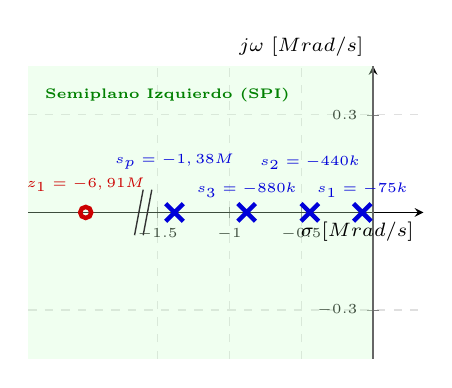
\begin{tikzpicture}
  \begin{axis}[
    width=6.6cm, height=5.3cm,
    axis lines=middle,
    xlabel={$\sigma$ [$\text{Mrad/s}$]},
    ylabel={$j\omega$ [$\text{Mrad/s}$]},
    xlabel style={at={(ticklabel* cs:1)}, anchor=north east, font=\scriptsize},
    ylabel style={at={(ticklabel* cs:1)}, anchor=south east, font=\scriptsize},
    xmin=-2.4, xmax=0.35, ymin=-0.45, ymax=0.45,
    xtick={-1.5, -1.0, -0.5, 0},
    ytick={-0.3, 0.3},
    grid=both, grid style={gray!25, dashed},
    tick label style={font=\tiny},
  ]
    % Zona estable LHP sombreada sutilmente
    \fill[green!20, opacity=0.3] (axis cs:-2.4,-0.45) rectangle (axis cs:0,0.45);

    % Eje jw (frontera de estabilidad)
    \draw[line width=1.0pt, black!60] (axis cs:0,-0.45) -- (axis cs:0,0.45);

    % Polos de G_aa(s) (cruces)
    \addplot[only marks, mark=x, mark size=4.5pt, line width=1.6pt, blue!85!black]
      coordinates {(-0.075, 0) (-0.440, 0) (-0.880, 0) (-1.382, 0)};

    \node[above=2pt, blue!85!black, font=\tiny\bfseries] at (axis cs:-0.075, 0) {$s_1 = -75\text{k}$};
    \node[above=12pt, blue!85!black, font=\tiny\bfseries] at (axis cs:-0.440, 0) {$s_2 = -440\text{k}$};
    \node[above=2pt, blue!85!black, font=\tiny\bfseries] at (axis cs:-0.880, 0) {$s_3 = -880\text{k}$};
    \node[above=12pt, blue!85!black, font=\tiny\bfseries] at (axis cs:-1.382, 0) {$s_p = -1,38\text{M}$};

    % Rotura de eje (axis break //)
    \draw[line width=0.5pt, black!80] (axis cs:-1.66, -0.07) -- (axis cs:-1.60, 0.07);
    \draw[line width=0.5pt, black!80] (axis cs:-1.60, -0.07) -- (axis cs:-1.54, 0.07);

    % Cero z1 como circulito sobre el eje
    \addplot[only marks, mark=o, mark size=2pt, line width=1.6pt, red!80!black]
      coordinates {(-2.0, 0)};
    \node[above=4pt, red!80!black, font=\tiny\bfseries, anchor=south] at (axis cs:-2.0, 0) {$z_1 = -6,91\text{M}$};

    \node[green!50!black, font=\tiny\bfseries, anchor=west] at (axis cs:-2.35, 0.36) {Semiplano Izquierdo (SPI)};
  \end{axis}
\end{tikzpicture}
